\documentclass[aspectratio=169, 11pt]{beamer}

\usepackage[T1]{fontenc}
\usepackage[utf8]{inputenc}
\usepackage{helvet}
\renewcommand{\familydefault}{\sfdefault}
\usepackage{xcolor}
\usepackage{tikz}
\usetikzlibrary{arrows.meta, positioning, fit, calc, shapes.geometric}
\usepackage{booktabs}
\usepackage{microtype}

\definecolor{kblue}{HTML}{00539F}
\definecolor{kbluedark}{HTML}{003D7A}
\definecolor{kbluelight}{HTML}{E8F2FB}
\definecolor{kbluepale}{HTML}{F4F8FC}
\definecolor{kvideogray}{HTML}{C8D0D8}
\definecolor{kscreenbg}{HTML}{EEF2F7}
\definecolor{korange}{HTML}{E87722}
\definecolor{kgreen}{HTML}{2E8B57}
\definecolor{kgray}{HTML}{6C757D}
\definecolor{klightgray}{HTML}{F0F2F4}

\usetheme{default}
\setbeamercolor{background canvas}{bg=white}
\setbeamercolor{frametitle}{fg=white, bg=kblue}
\setbeamerfont{frametitle}{size=\large, series=\bfseries, family=\sffamily}
\setbeamertemplate{navigation symbols}{}
\setbeamertemplate{footline}{%
  \hfill\tiny\color{kgray}\insertframenumber\hspace{6pt}\vspace{4pt}%
}
\setbeamertemplate{frametitle}{%
  \begin{beamercolorbox}[wd=\paperwidth, ht=0.65cm, dp=0.15cm, leftskip=0.4cm]{frametitle}%
    \usebeamerfont{frametitle}\insertframetitle%
  \end{beamercolorbox}%
}

\tikzset{
  farrow/.style={-{Stealth[length=4pt, width=3pt]}, kgray, line width=0.5pt},
}

\begin{document}

{
\setbeamercolor{background canvas}{bg=kgreen!60!black}
\setbeamertemplate{footline}{}
\begin{frame}
\begin{tikzpicture}[remember picture, overlay]
  \node[anchor=north west, font=\fontsize{24}{28}\selectfont\sffamily\bfseries, text=white]
    at ($(current page.north west)+(1.0,-1.2)$) {NPR --- Nonphotorealistic Rendering};
  \node[anchor=north west, font=\large\sffamily, text=white!75]
    at ($(current page.north west)+(1.0,-2.3)$) {Article Summaries --- Section 3};
  \draw[white!40, line width=0.5pt] ($(current page.north west)+(1.0,-3.0)$)
    -- ($(current page.north west)+(14.0,-3.0)$);
  \node[anchor=north west, font=\small\sffamily, text=white!80]
    at ($(current page.north west)+(1.0,-3.4)$) {Gooch 1998 \textbullet{} Lake 2000 \textbullet{} Isenberg 2003 \textbullet{} Gonzalez \& Woods 2018 \textbullet{} Marr \& Hildreth 1980 \textbullet{} Canny 1986 \textbullet{} Barla 2006};
  \node[anchor=north west, font=\small\sffamily, text=white!80]
    at ($(current page.north west)+(1.0,-4.1)$) {Kyprianidis 2009 \textbullet{} Praun 2001 \textbullet{} Roberts 1963 \textbullet{} Kumar \& Poornima 2019 \textbullet{} Wisessing 2016 \textbullet{} Wisessing 2020};
  \node[anchor=north west, font=\small\sffamily, text=white!80]
    at ($(current page.north west)+(1.0,-4.8)$) {Petikam 2021 \textbullet{} Riefard 2024 \textbullet{} Roshaan 2026 (AHEAD)};
  \node[anchor=south west, font=\small\sffamily, text=white!60]
    at ($(current page.south west)+(1.0,0.5)$)
    {Nidanur G\"unay \quad\textbullet\quad University of Konstanz \quad\textbullet\quad 2026};
\end{tikzpicture}
\end{frame}
}

%% ═══════════════════════════════════════════════════════════════════════════
%% Gooch et al. 1998
%% ═══════════════════════════════════════════════════════════════════════════
\begin{frame}{Gooch et al. (1998) \textnormal{\normalsize --- A Nonphotorealistic Lighting Model for Technical Illustration}}
\begin{center}
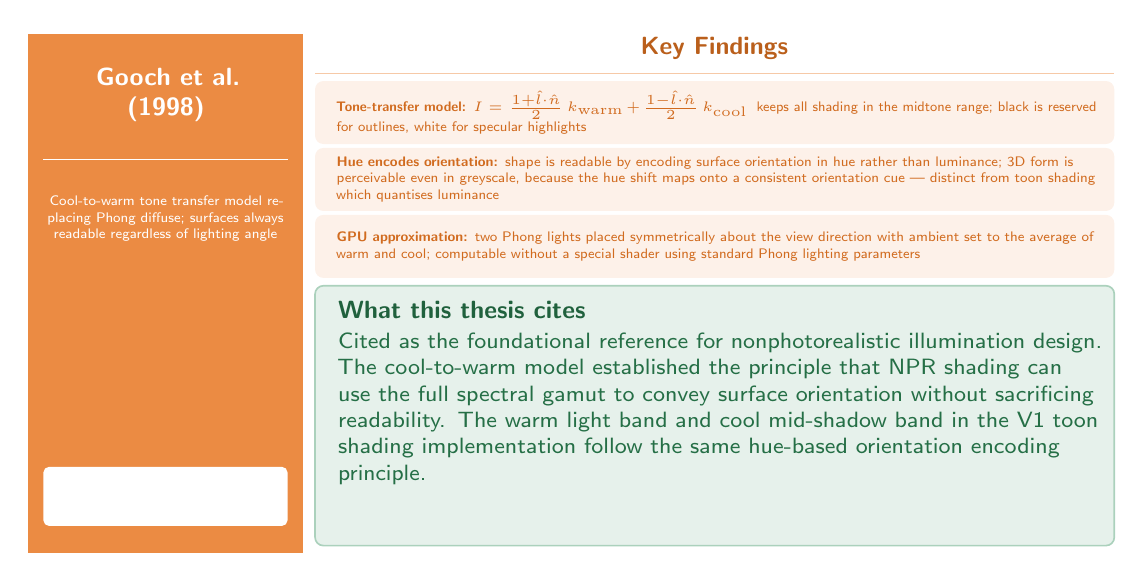
\begin{tikzpicture}[x=1cm, y=1cm]
\fill[korange!85] (0.0,0.0) rectangle (3.5,6.6);
\node[font=\small\sffamily\bfseries, text=white, align=center, text width=3.1cm]
  at (1.75,5.82) {Gooch et al.\\(1998)};
\draw[white!30, line width=0.3pt] (0.2,5.00) -- (3.3,5.00);
\node[font=\tiny\sffamily, text=white!85, align=center, text width=3.0cm]
  at (1.75,4.25) {Cool-to-warm tone transfer model replacing Phong diffuse; surfaces always readable regardless of lighting angle};
\fill[white!20, rounded corners=2pt] (0.2,0.35) rectangle (3.3,1.10);
\node[font=\tiny\sffamily\bfseries, text=white, align=center]
  at (1.75,0.72) {SIGGRAPH 1998\\technical illustration};
\node[font=\small\sffamily\bfseries\color{korange!80!black}] at (8.72,6.42) {Key Findings};
\draw[korange!40, line width=0.3pt] (3.65,6.10) -- (13.8,6.10);
\fill[korange!10, rounded corners=3pt] (3.65,5.20) rectangle (13.8,6.00);
\node[font=\tiny\sffamily\color{korange!90!black}, anchor=west, text width=9.65cm]
  at (3.80,5.60) {\textbf{Tone-transfer model:} $I = \frac{1+\hat{l}\cdot\hat{n}}{2}\,k_{\mathrm{warm}} + \frac{1-\hat{l}\cdot\hat{n}}{2}\,k_{\mathrm{cool}}$\; keeps all shading in the midtone range; black is reserved for outlines, white for specular highlights};
\fill[korange!10, rounded corners=3pt] (3.65,4.35) rectangle (13.8,5.15);
\node[font=\tiny\sffamily\color{korange!90!black}, anchor=west, text width=9.65cm]
  at (3.80,4.75) {\textbf{Hue encodes orientation:} shape is readable by encoding surface orientation in hue rather than luminance; 3D form is perceivable even in greyscale, because the hue shift maps onto a consistent orientation cue --- distinct from toon shading which quantises luminance};
\fill[korange!10, rounded corners=3pt] (3.65,3.50) rectangle (13.8,4.30);
\node[font=\tiny\sffamily\color{korange!90!black}, anchor=west, text width=9.65cm]
  at (3.80,3.90) {\textbf{GPU approximation:} two Phong lights placed symmetrically about the view direction with ambient set to the average of warm and cool; computable without a special shader using standard Phong lighting parameters};
\fill[kgreen!12, draw=kgreen!40, rounded corners=3pt, line width=0.6pt]
  (3.65,0.1) rectangle (13.8,3.40);
\node[font=\small\sffamily\bfseries\color{kgreen!70!black}, anchor=west]
  at (3.82,3.1) {What this thesis cites};
\node[font=\footnotesize\sffamily\color{kgreen!80!black}, anchor=north west, text width=9.65cm]
  at (3.82,2.92) {Cited as the foundational reference for nonphotorealistic illumination design. The cool-to-warm model established the principle that NPR shading can use the full spectral gamut to convey surface orientation without sacrificing readability. The warm light band and cool mid-shadow band in the V1 toon shading implementation follow the same hue-based orientation encoding principle.};
\end{tikzpicture}
\end{center}
\end{frame}

%% ═══════════════════════════════════════════════════════════════════════════
%% Lake et al. 2000
%% ═══════════════════════════════════════════════════════════════════════════
\begin{frame}{Lake et al. (2000) \textnormal{\normalsize --- Stylized Rendering for Real-Time 3D Animation}}
\begin{center}
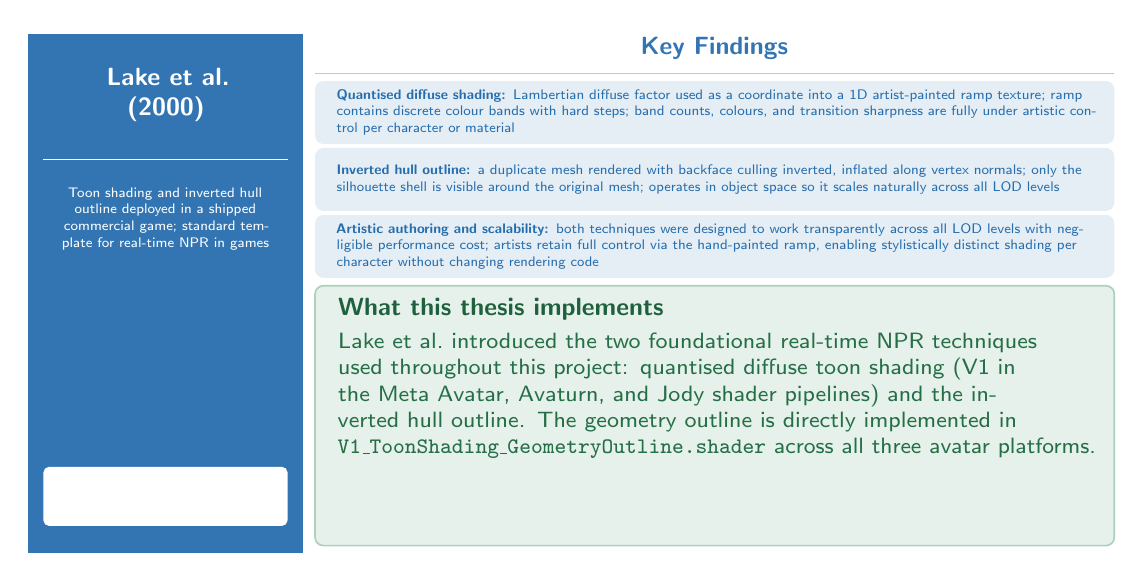
\begin{tikzpicture}[x=1cm, y=1cm]
\fill[kblue!80] (0.0,0.0) rectangle (3.5,6.6);
\node[font=\small\sffamily\bfseries, text=white, align=center, text width=3.1cm]
  at (1.75,5.82) {Lake et al.\\(2000)};
\draw[white!30, line width=0.3pt] (0.2,5.00) -- (3.3,5.00);
\node[font=\tiny\sffamily, text=white!85, align=center, text width=3.0cm]
  at (1.75,4.25) {Toon shading and inverted hull outline deployed in a shipped commercial game; standard template for real-time NPR in games};
\fill[white!20, rounded corners=2pt] (0.2,0.35) rectangle (3.3,1.10);
\node[font=\tiny\sffamily\bfseries, text=white, align=center]
  at (1.75,0.72) {NPAR 2000\\Shiny Entertainment};
\node[font=\small\sffamily\bfseries\color{kblue!80}] at (8.72,6.42) {Key Findings};
\draw[kblue!30, line width=0.3pt] (3.65,6.10) -- (13.8,6.10);
\fill[kblue!10, rounded corners=3pt] (3.65,5.20) rectangle (13.8,6.00);
\node[font=\tiny\sffamily\color{kblue!85}, anchor=west, text width=9.65cm]
  at (3.80,5.60) {\textbf{Quantised diffuse shading:} Lambertian diffuse factor used as a coordinate into a 1D artist-painted ramp texture; ramp contains discrete colour bands with hard steps; band counts, colours, and transition sharpness are fully under artistic control per character or material};
\fill[kblue!10, rounded corners=3pt] (3.65,4.35) rectangle (13.8,5.15);
\node[font=\tiny\sffamily\color{kblue!85}, anchor=west, text width=9.65cm]
  at (3.80,4.75) {\textbf{Inverted hull outline:} a duplicate mesh rendered with backface culling inverted, inflated along vertex normals; only the silhouette shell is visible around the original mesh; operates in object space so it scales naturally across all LOD levels};
\fill[kblue!10, rounded corners=3pt] (3.65,3.50) rectangle (13.8,4.30);
\node[font=\tiny\sffamily\color{kblue!85}, anchor=west, text width=9.65cm]
  at (3.80,3.90) {\textbf{Artistic authoring and scalability:} both techniques were designed to work transparently across all LOD levels with negligible performance cost; artists retain full control via the hand-painted ramp, enabling stylistically distinct shading per character without changing rendering code};
\fill[kgreen!12, draw=kgreen!40, rounded corners=3pt, line width=0.6pt]
  (3.65,0.1) rectangle (13.8,3.40);
\node[font=\small\sffamily\bfseries\color{kgreen!70!black}, anchor=west]
  at (3.82,3.1) {What this thesis implements};
\node[font=\footnotesize\sffamily\color{kgreen!80!black}, anchor=north west, text width=9.65cm]
  at (3.82,2.92) {Lake et al.\ introduced the two foundational real-time NPR techniques used throughout this project: quantised diffuse toon shading (V1 in the Meta Avatar, Avaturn, and Jody shader pipelines) and the inverted hull outline. The geometry outline is directly implemented in \texttt{V1\_ToonShading\_GeometryOutline.shader} across all three avatar platforms.};
\end{tikzpicture}
\end{center}
\end{frame}

%% ═══════════════════════════════════════════════════════════════════════════
%% Isenberg et al. 2003
%% ═══════════════════════════════════════════════════════════════════════════
\begin{frame}{Isenberg et al. (2003) \textnormal{\normalsize --- A Developer's Guide to Silhouette Algorithms}}
\begin{center}
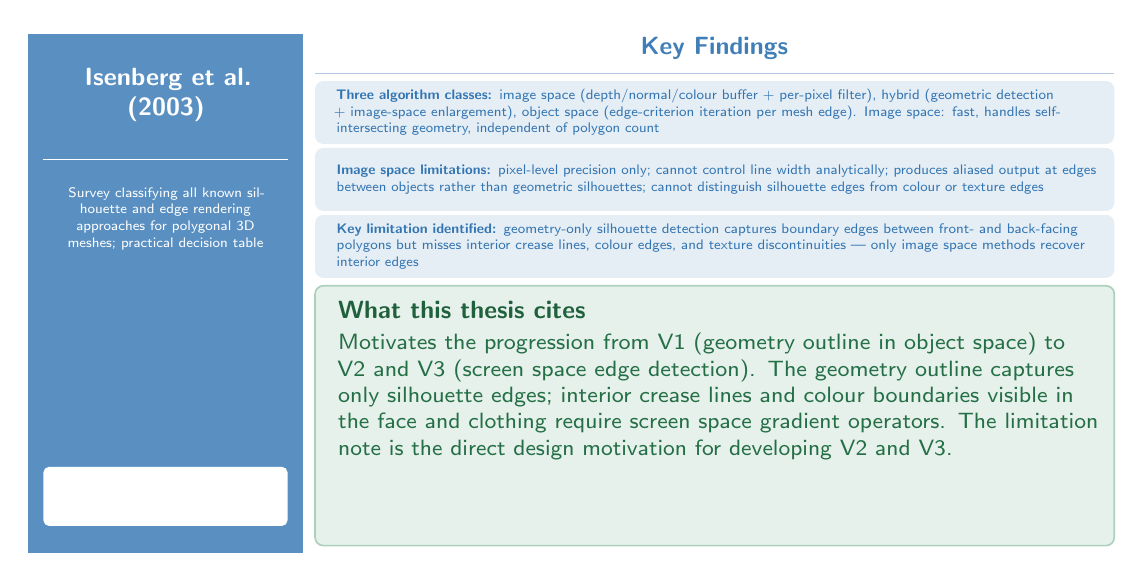
\begin{tikzpicture}[x=1cm, y=1cm]
\fill[kblue!65] (0.0,0.0) rectangle (3.5,6.6);
\node[font=\small\sffamily\bfseries, text=white, align=center, text width=3.1cm]
  at (1.75,5.82) {Isenberg et al.\\(2003)};
\draw[white!30, line width=0.3pt] (0.2,5.00) -- (3.3,5.00);
\node[font=\tiny\sffamily, text=white!85, align=center, text width=3.0cm]
  at (1.75,4.25) {Survey classifying all known silhouette and edge rendering approaches for polygonal 3D meshes; practical decision table};
\fill[white!20, rounded corners=2pt] (0.2,0.35) rectangle (3.3,1.10);
\node[font=\tiny\sffamily\bfseries, text=white, align=center]
  at (1.75,0.72) {IEEE CG\&A survey\\2003};
\node[font=\small\sffamily\bfseries\color{kblue!75}] at (8.72,6.42) {Key Findings};
\draw[kblue!30, line width=0.3pt] (3.65,6.10) -- (13.8,6.10);
\fill[kblue!10, rounded corners=3pt] (3.65,5.20) rectangle (13.8,6.00);
\node[font=\tiny\sffamily\color{kblue!80}, anchor=west, text width=9.65cm]
  at (3.80,5.60) {\textbf{Three algorithm classes:} image space (depth/normal/colour buffer + per-pixel filter), hybrid (geometric detection + image-space enlargement), object space (edge-criterion iteration per mesh edge). Image space: fast, handles self-intersecting geometry, independent of polygon count};
\fill[kblue!10, rounded corners=3pt] (3.65,4.35) rectangle (13.8,5.15);
\node[font=\tiny\sffamily\color{kblue!80}, anchor=west, text width=9.65cm]
  at (3.80,4.75) {\textbf{Image space limitations:} pixel-level precision only; cannot control line width analytically; produces aliased output at edges between objects rather than geometric silhouettes; cannot distinguish silhouette edges from colour or texture edges};
\fill[kblue!10, rounded corners=3pt] (3.65,3.50) rectangle (13.8,4.30);
\node[font=\tiny\sffamily\color{kblue!80}, anchor=west, text width=9.65cm]
  at (3.80,3.90) {\textbf{Key limitation identified:} geometry-only silhouette detection captures boundary edges between front- and back-facing polygons but misses interior crease lines, colour edges, and texture discontinuities --- only image space methods recover interior edges};
\fill[kgreen!12, draw=kgreen!40, rounded corners=3pt, line width=0.6pt]
  (3.65,0.1) rectangle (13.8,3.40);
\node[font=\small\sffamily\bfseries\color{kgreen!70!black}, anchor=west]
  at (3.82,3.1) {What this thesis cites};
\node[font=\footnotesize\sffamily\color{kgreen!80!black}, anchor=north west, text width=9.65cm]
  at (3.82,2.92) {Motivates the progression from V1 (geometry outline in object space) to V2 and V3 (screen space edge detection). The geometry outline captures only silhouette edges; interior crease lines and colour boundaries visible in the face and clothing require screen space gradient operators. The limitation note is the direct design motivation for developing V2 and V3.};
\end{tikzpicture}
\end{center}
\end{frame}

%% ═══════════════════════════════════════════════════════════════════════════
%% Gonzalez & Woods 2018
%% ═══════════════════════════════════════════════════════════════════════════
\begin{frame}{Gonzalez \& Woods (2018) \textnormal{\normalsize --- Digital Image Processing (4th edition)}}
\begin{center}
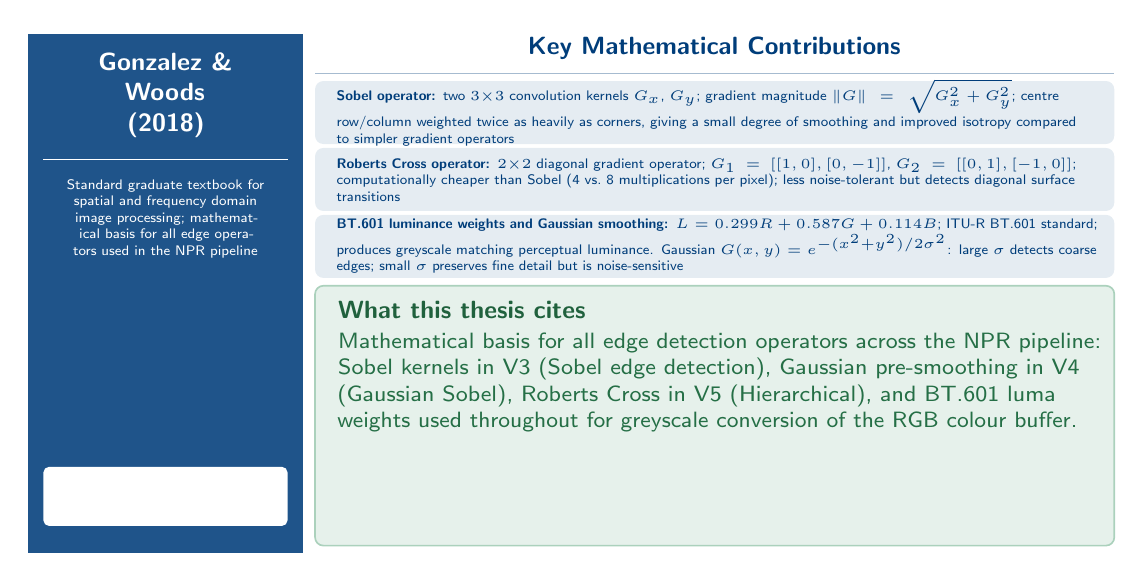
\begin{tikzpicture}[x=1cm, y=1cm]
\fill[kbluedark!88] (0.0,0.0) rectangle (3.5,6.6);
\node[font=\small\sffamily\bfseries, text=white, align=center, text width=3.1cm]
  at (1.75,5.82) {Gonzalez \&\\Woods\\(2018)};
\draw[white!30, line width=0.3pt] (0.2,5.00) -- (3.3,5.00);
\node[font=\tiny\sffamily, text=white!85, align=center, text width=3.0cm]
  at (1.75,4.25) {Standard graduate textbook for spatial and frequency domain image processing; mathematical basis for all edge operators used in the NPR pipeline};
\fill[white!20, rounded corners=2pt] (0.2,0.35) rectangle (3.3,1.10);
\node[font=\tiny\sffamily\bfseries, text=white, align=center]
  at (1.75,0.72) {Textbook\\Pearson / Prentice Hall};
\node[font=\small\sffamily\bfseries\color{kbluedark}] at (8.72,6.42) {Key Mathematical Contributions};
\draw[kbluedark!35, line width=0.3pt] (3.65,6.10) -- (13.8,6.10);
\fill[kbluedark!10, rounded corners=3pt] (3.65,5.20) rectangle (13.8,6.00);
\node[font=\tiny\sffamily\color{kbluedark}, anchor=west, text width=9.65cm]
  at (3.80,5.60) {\textbf{Sobel operator:} two $3{\times}3$ convolution kernels $G_x$, $G_y$; gradient magnitude $\|G\| = \sqrt{G_x^2+G_y^2}$; centre row/column weighted twice as heavily as corners, giving a small degree of smoothing and improved isotropy compared to simpler gradient operators};
\fill[kbluedark!10, rounded corners=3pt] (3.65,4.35) rectangle (13.8,5.15);
\node[font=\tiny\sffamily\color{kbluedark}, anchor=west, text width=9.65cm]
  at (3.80,4.75) {\textbf{Roberts Cross operator:} $2{\times}2$ diagonal gradient operator; $G_1 = [[1,0],[0,-1]]$, $G_2 = [[0,1],[-1,0]]$; computationally cheaper than Sobel (4 vs.\ 8 multiplications per pixel); less noise-tolerant but detects diagonal surface transitions};
\fill[kbluedark!10, rounded corners=3pt] (3.65,3.50) rectangle (13.8,4.30);
\node[font=\tiny\sffamily\color{kbluedark}, anchor=west, text width=9.65cm]
  at (3.80,3.90) {\textbf{BT.601 luminance weights and Gaussian smoothing:} $L = 0.299R + 0.587G + 0.114B$; ITU-R BT.601 standard; produces greyscale matching perceptual luminance. Gaussian $G(x,y) = e^{-(x^2+y^2)/2\sigma^2}$: large $\sigma$ detects coarse edges; small $\sigma$ preserves fine detail but is noise-sensitive};
\fill[kgreen!12, draw=kgreen!40, rounded corners=3pt, line width=0.6pt]
  (3.65,0.1) rectangle (13.8,3.40);
\node[font=\small\sffamily\bfseries\color{kgreen!70!black}, anchor=west]
  at (3.82,3.1) {What this thesis cites};
\node[font=\footnotesize\sffamily\color{kgreen!80!black}, anchor=north west, text width=9.65cm]
  at (3.82,2.92) {Mathematical basis for all edge detection operators across the NPR pipeline: Sobel kernels in V3 (Sobel edge detection), Gaussian pre-smoothing in V4 (Gaussian Sobel), Roberts Cross in V5 (Hierarchical), and BT.601 luma weights used throughout for greyscale conversion of the RGB colour buffer.};
\end{tikzpicture}
\end{center}
\end{frame}

%% ═══════════════════════════════════════════════════════════════════════════
%% Marr & Hildreth 1980
%% ═══════════════════════════════════════════════════════════════════════════
\begin{frame}{Marr \& Hildreth (1980) \textnormal{\normalsize --- Theory of Edge Detection}}
\begin{center}
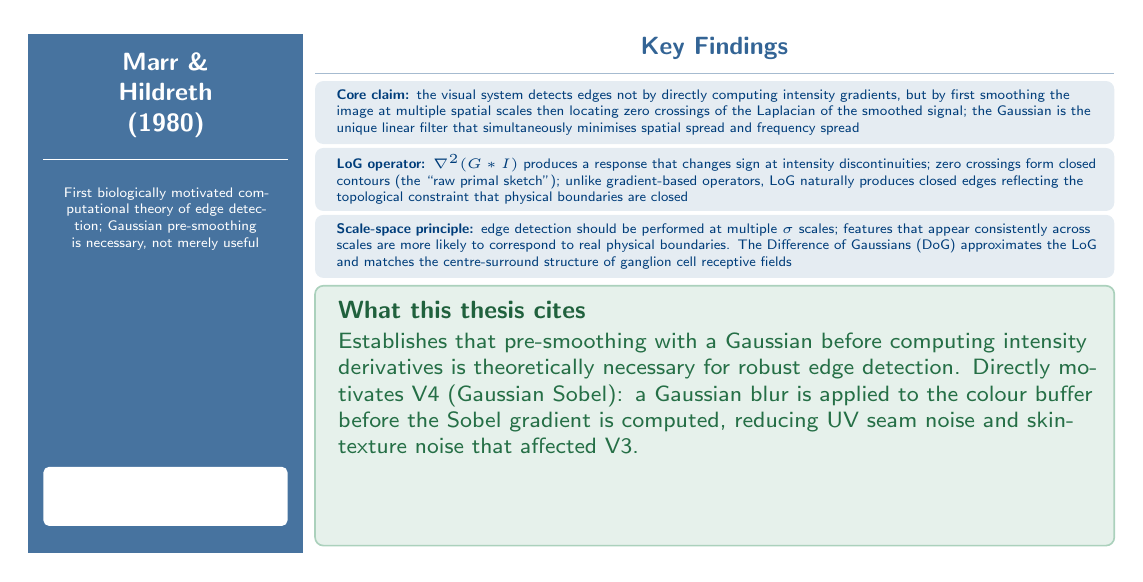
\begin{tikzpicture}[x=1cm, y=1cm]
\fill[kbluedark!72] (0.0,0.0) rectangle (3.5,6.6);
\node[font=\small\sffamily\bfseries, text=white, align=center, text width=3.1cm]
  at (1.75,5.82) {Marr \&\\Hildreth\\(1980)};
\draw[white!30, line width=0.3pt] (0.2,5.00) -- (3.3,5.00);
\node[font=\tiny\sffamily, text=white!85, align=center, text width=3.0cm]
  at (1.75,4.25) {First biologically motivated computational theory of edge detection; Gaussian pre-smoothing is necessary, not merely useful};
\fill[white!20, rounded corners=2pt] (0.2,0.35) rectangle (3.3,1.10);
\node[font=\tiny\sffamily\bfseries, text=white, align=center]
  at (1.75,0.72) {Proc. Royal Society B\\theoretical};
\node[font=\small\sffamily\bfseries\color{kbluedark!80}] at (8.72,6.42) {Key Findings};
\draw[kbluedark!35, line width=0.3pt] (3.65,6.10) -- (13.8,6.10);
\fill[kbluedark!10, rounded corners=3pt] (3.65,5.20) rectangle (13.8,6.00);
\node[font=\tiny\sffamily\color{kbluedark}, anchor=west, text width=9.65cm]
  at (3.80,5.60) {\textbf{Core claim:} the visual system detects edges not by directly computing intensity gradients, but by first smoothing the image at multiple spatial scales then locating zero crossings of the Laplacian of the smoothed signal; the Gaussian is the unique linear filter that simultaneously minimises spatial spread and frequency spread};
\fill[kbluedark!10, rounded corners=3pt] (3.65,4.35) rectangle (13.8,5.15);
\node[font=\tiny\sffamily\color{kbluedark}, anchor=west, text width=9.65cm]
  at (3.80,4.75) {\textbf{LoG operator:} $\nabla^2(G*I)$ produces a response that changes sign at intensity discontinuities; zero crossings form closed contours (the ``raw primal sketch''); unlike gradient-based operators, LoG naturally produces closed edges reflecting the topological constraint that physical boundaries are closed};
\fill[kbluedark!10, rounded corners=3pt] (3.65,3.50) rectangle (13.8,4.30);
\node[font=\tiny\sffamily\color{kbluedark}, anchor=west, text width=9.65cm]
  at (3.80,3.90) {\textbf{Scale-space principle:} edge detection should be performed at multiple $\sigma$ scales; features that appear consistently across scales are more likely to correspond to real physical boundaries. The Difference of Gaussians (DoG) approximates the LoG and matches the centre-surround structure of ganglion cell receptive fields};
\fill[kgreen!12, draw=kgreen!40, rounded corners=3pt, line width=0.6pt]
  (3.65,0.1) rectangle (13.8,3.40);
\node[font=\small\sffamily\bfseries\color{kgreen!70!black}, anchor=west]
  at (3.82,3.1) {What this thesis cites};
\node[font=\footnotesize\sffamily\color{kgreen!80!black}, anchor=north west, text width=9.65cm]
  at (3.82,2.92) {Establishes that pre-smoothing with a Gaussian before computing intensity derivatives is theoretically necessary for robust edge detection. Directly motivates V4 (Gaussian Sobel): a Gaussian blur is applied to the colour buffer before the Sobel gradient is computed, reducing UV seam noise and skin-texture noise that affected V3.};
\end{tikzpicture}
\end{center}
\end{frame}

%% ═══════════════════════════════════════════════════════════════════════════
%% Canny 1986
%% ═══════════════════════════════════════════════════════════════════════════
\begin{frame}{Canny (1986) \textnormal{\normalsize --- A Computational Approach to Edge Detection}}
\begin{center}
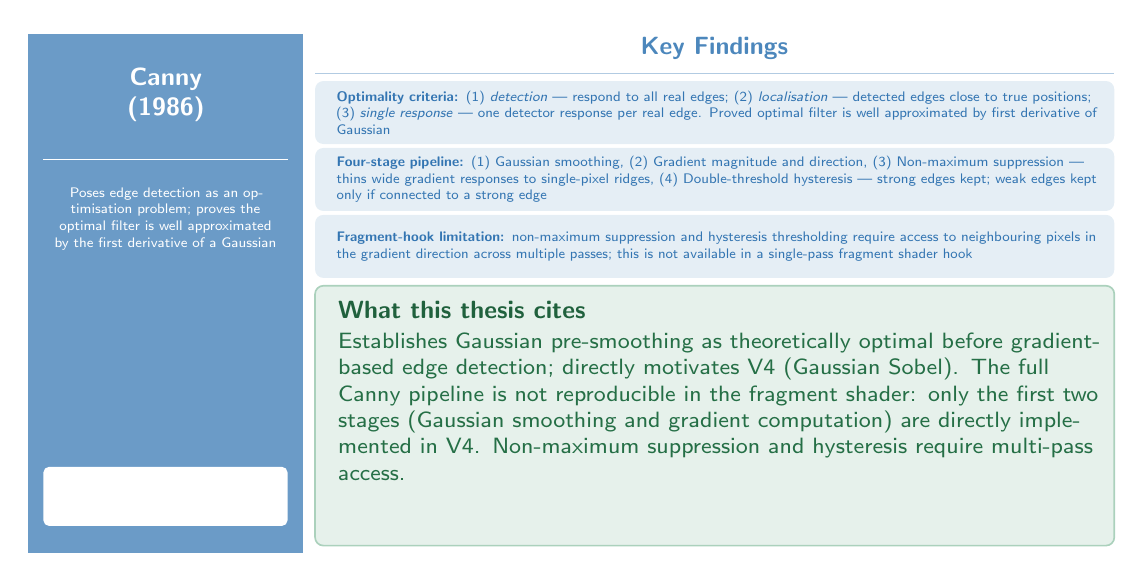
\begin{tikzpicture}[x=1cm, y=1cm]
\fill[kblue!58] (0.0,0.0) rectangle (3.5,6.6);
\node[font=\small\sffamily\bfseries, text=white, align=center, text width=3.1cm]
  at (1.75,5.82) {Canny\\(1986)};
\draw[white!30, line width=0.3pt] (0.2,5.00) -- (3.3,5.00);
\node[font=\tiny\sffamily, text=white!85, align=center, text width=3.0cm]
  at (1.75,4.25) {Poses edge detection as an optimisation problem; proves the optimal filter is well approximated by the first derivative of a Gaussian};
\fill[white!20, rounded corners=2pt] (0.2,0.35) rectangle (3.3,1.10);
\node[font=\tiny\sffamily\bfseries, text=white, align=center]
  at (1.75,0.72) {IEEE TPAMI\\4-stage pipeline};
\node[font=\small\sffamily\bfseries\color{kblue!70}] at (8.72,6.42) {Key Findings};
\draw[kblue!30, line width=0.3pt] (3.65,6.10) -- (13.8,6.10);
\fill[kblue!10, rounded corners=3pt] (3.65,5.20) rectangle (13.8,6.00);
\node[font=\tiny\sffamily\color{kblue!80}, anchor=west, text width=9.65cm]
  at (3.80,5.60) {\textbf{Optimality criteria:} (1) \textit{detection} --- respond to all real edges; (2) \textit{localisation} --- detected edges close to true positions; (3) \textit{single response} --- one detector response per real edge. Proved optimal filter is well approximated by first derivative of Gaussian};
\fill[kblue!10, rounded corners=3pt] (3.65,4.35) rectangle (13.8,5.15);
\node[font=\tiny\sffamily\color{kblue!80}, anchor=west, text width=9.65cm]
  at (3.80,4.75) {\textbf{Four-stage pipeline:} (1) Gaussian smoothing, (2) Gradient magnitude and direction, (3) Non-maximum suppression --- thins wide gradient responses to single-pixel ridges, (4) Double-threshold hysteresis --- strong edges kept; weak edges kept only if connected to a strong edge};
\fill[kblue!10, rounded corners=3pt] (3.65,3.50) rectangle (13.8,4.30);
\node[font=\tiny\sffamily\color{kblue!80}, anchor=west, text width=9.65cm]
  at (3.80,3.90) {\textbf{Fragment-hook limitation:} non-maximum suppression and hysteresis thresholding require access to neighbouring pixels in the gradient direction across multiple passes; this is not available in a single-pass fragment shader hook};
\fill[kgreen!12, draw=kgreen!40, rounded corners=3pt, line width=0.6pt]
  (3.65,0.1) rectangle (13.8,3.40);
\node[font=\small\sffamily\bfseries\color{kgreen!70!black}, anchor=west]
  at (3.82,3.1) {What this thesis cites};
\node[font=\footnotesize\sffamily\color{kgreen!80!black}, anchor=north west, text width=9.65cm]
  at (3.82,2.92) {Establishes Gaussian pre-smoothing as theoretically optimal before gradient-based edge detection; directly motivates V4 (Gaussian Sobel). The full Canny pipeline is not reproducible in the fragment shader: only the first two stages (Gaussian smoothing and gradient computation) are directly implemented in V4. Non-maximum suppression and hysteresis require multi-pass access.};
\end{tikzpicture}
\end{center}
\end{frame}

%% ═══════════════════════════════════════════════════════════════════════════
%% Barla et al. 2006 — X-Toon
%% ═══════════════════════════════════════════════════════════════════════════
\begin{frame}{Barla et al. (2006) \textnormal{\normalsize --- X-Toon: An Extended Toon Shader}}
\begin{center}
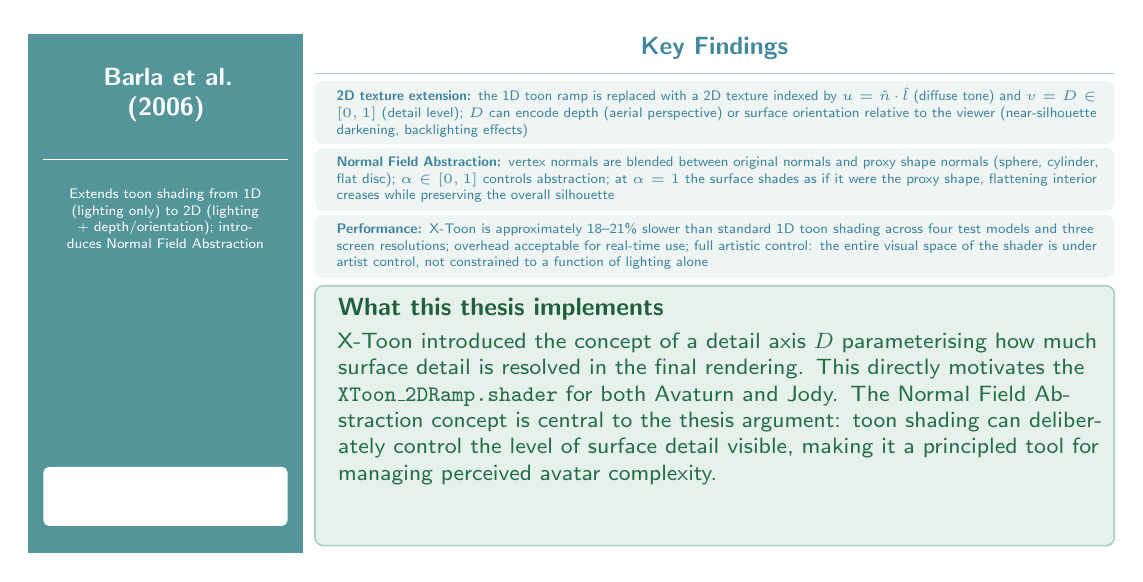
\begin{tikzpicture}[x=1cm, y=1cm]
\fill[kblue!45!kgreen!75] (0.0,0.0) rectangle (3.5,6.6);
\node[font=\small\sffamily\bfseries, text=white, align=center, text width=3.1cm]
  at (1.75,5.82) {Barla et al.\\(2006)};
\draw[white!30, line width=0.3pt] (0.2,5.00) -- (3.3,5.00);
\node[font=\tiny\sffamily, text=white!85, align=center, text width=3.0cm]
  at (1.75,4.25) {Extends toon shading from 1D (lighting only) to 2D (lighting + depth/orientation); introduces Normal Field Abstraction};
\fill[white!20, rounded corners=2pt] (0.2,0.35) rectangle (3.3,1.10);
\node[font=\tiny\sffamily\bfseries, text=white, align=center]
  at (1.75,0.72) {NPAR 2006\\X-Toon shader};
\node[font=\small\sffamily\bfseries\color{kblue!60!kgreen!80}] at (8.72,6.42) {Key Findings};
\draw[kblue!30!kgreen!40, line width=0.3pt] (3.65,6.10) -- (13.8,6.10);
\fill[kblue!8!kgreen!8, rounded corners=3pt] (3.65,5.20) rectangle (13.8,6.00);
\node[font=\tiny\sffamily\color{kblue!70!kgreen!80}, anchor=west, text width=9.65cm]
  at (3.80,5.60) {\textbf{2D texture extension:} the 1D toon ramp is replaced with a 2D texture indexed by $u = \hat{n}\cdot\hat{l}$ (diffuse tone) and $v = D \in [0,1]$ (detail level); $D$ can encode depth (aerial perspective) or surface orientation relative to the viewer (near-silhouette darkening, backlighting effects)};
\fill[kblue!8!kgreen!8, rounded corners=3pt] (3.65,4.35) rectangle (13.8,5.15);
\node[font=\tiny\sffamily\color{kblue!70!kgreen!80}, anchor=west, text width=9.65cm]
  at (3.80,4.75) {\textbf{Normal Field Abstraction:} vertex normals are blended between original normals and proxy shape normals (sphere, cylinder, flat disc); $\alpha \in [0,1]$ controls abstraction; at $\alpha=1$ the surface shades as if it were the proxy shape, flattening interior creases while preserving the overall silhouette};
\fill[kblue!8!kgreen!8, rounded corners=3pt] (3.65,3.50) rectangle (13.8,4.30);
\node[font=\tiny\sffamily\color{kblue!70!kgreen!80}, anchor=west, text width=9.65cm]
  at (3.80,3.90) {\textbf{Performance:} X-Toon is approximately 18--21\% slower than standard 1D toon shading across four test models and three screen resolutions; overhead acceptable for real-time use; full artistic control: the entire visual space of the shader is under artist control, not constrained to a function of lighting alone};
\fill[kgreen!12, draw=kgreen!40, rounded corners=3pt, line width=0.6pt]
  (3.65,0.1) rectangle (13.8,3.40);
\node[font=\small\sffamily\bfseries\color{kgreen!70!black}, anchor=west]
  at (3.82,3.1) {What this thesis implements};
\node[font=\footnotesize\sffamily\color{kgreen!80!black}, anchor=north west, text width=9.65cm]
  at (3.82,2.92) {X-Toon introduced the concept of a detail axis $D$ parameterising how much surface detail is resolved in the final rendering. This directly motivates the \texttt{XToon\_2DRamp.shader} for both Avaturn and Jody. The Normal Field Abstraction concept is central to the thesis argument: toon shading can deliberately control the level of surface detail visible, making it a principled tool for managing perceived avatar complexity.};
\end{tikzpicture}
\end{center}
\end{frame}

%% ═══════════════════════════════════════════════════════════════════════════
%% Kyprianidis et al. 2009
%% ═══════════════════════════════════════════════════════════════════════════
\begin{frame}{Kyprianidis et al. (2009) \textnormal{\normalsize --- Image Abstraction by Anisotropic Kuwahara Filtering}}
\begin{center}
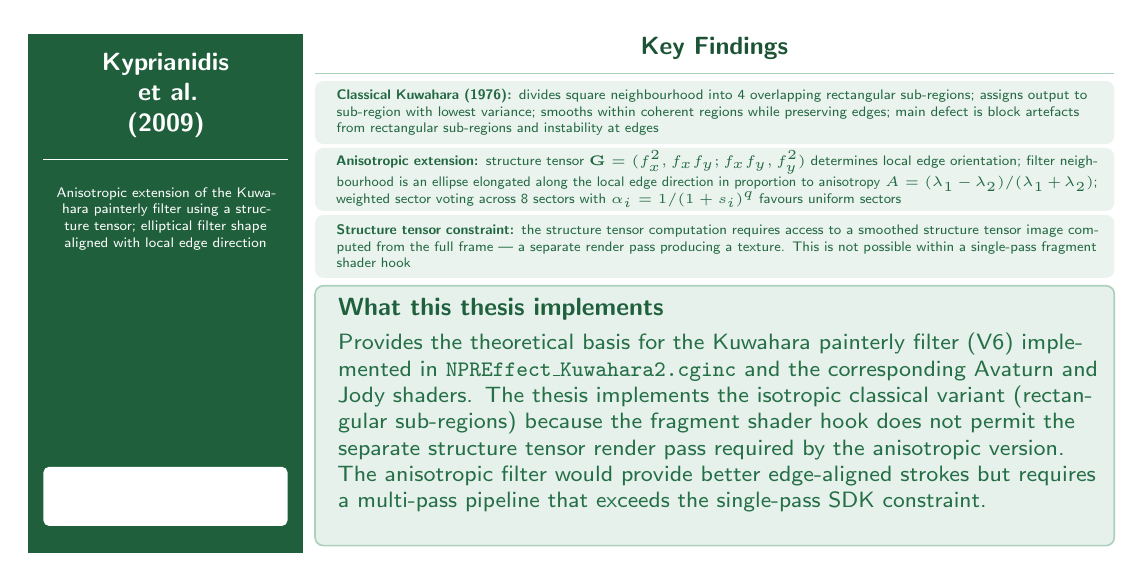
\begin{tikzpicture}[x=1cm, y=1cm]
\fill[kgreen!68!black] (0.0,0.0) rectangle (3.5,6.6);
\node[font=\small\sffamily\bfseries, text=white, align=center, text width=3.1cm]
  at (1.75,5.82) {Kyprianidis\\et al.\\(2009)};
\draw[white!30, line width=0.3pt] (0.2,5.00) -- (3.3,5.00);
\node[font=\tiny\sffamily, text=white!85, align=center, text width=3.0cm]
  at (1.75,4.25) {Anisotropic extension of the Kuwahara painterly filter using a structure tensor; elliptical filter shape aligned with local edge direction};
\fill[white!20, rounded corners=2pt] (0.2,0.35) rectangle (3.3,1.10);
\node[font=\tiny\sffamily\bfseries, text=white, align=center]
  at (1.75,0.72) {CGF Pacific Graphics\\GPU implementation};
\node[font=\small\sffamily\bfseries\color{kgreen!60!black}] at (8.72,6.42) {Key Findings};
\draw[kgreen!40, line width=0.3pt] (3.65,6.10) -- (13.8,6.10);
\fill[kgreen!10, rounded corners=3pt] (3.65,5.20) rectangle (13.8,6.00);
\node[font=\tiny\sffamily\color{kgreen!75!black}, anchor=west, text width=9.65cm]
  at (3.80,5.60) {\textbf{Classical Kuwahara (1976):} divides square neighbourhood into 4 overlapping rectangular sub-regions; assigns output to sub-region with lowest variance; smooths within coherent regions while preserving edges; main defect is block artefacts from rectangular sub-regions and instability at edges};
\fill[kgreen!10, rounded corners=3pt] (3.65,4.35) rectangle (13.8,5.15);
\node[font=\tiny\sffamily\color{kgreen!75!black}, anchor=west, text width=9.65cm]
  at (3.80,4.75) {\textbf{Anisotropic extension:} structure tensor $\mathbf{G} = (f_x^2, f_xf_y; f_xf_y, f_y^2)$ determines local edge orientation; filter neighbourhood is an ellipse elongated along the local edge direction in proportion to anisotropy $A = (\lambda_1-\lambda_2)/(\lambda_1+\lambda_2)$; weighted sector voting across 8 sectors with $\alpha_i = 1/(1+s_i)^q$ favours uniform sectors};
\fill[kgreen!10, rounded corners=3pt] (3.65,3.50) rectangle (13.8,4.30);
\node[font=\tiny\sffamily\color{kgreen!75!black}, anchor=west, text width=9.65cm]
  at (3.80,3.90) {\textbf{Structure tensor constraint:} the structure tensor computation requires access to a smoothed structure tensor image computed from the full frame --- a separate render pass producing a texture. This is not possible within a single-pass fragment shader hook};
\fill[kgreen!12, draw=kgreen!40, rounded corners=3pt, line width=0.6pt]
  (3.65,0.1) rectangle (13.8,3.40);
\node[font=\small\sffamily\bfseries\color{kgreen!70!black}, anchor=west]
  at (3.82,3.1) {What this thesis implements};
\node[font=\footnotesize\sffamily\color{kgreen!80!black}, anchor=north west, text width=9.65cm]
  at (3.82,2.92) {Provides the theoretical basis for the Kuwahara painterly filter (V6) implemented in \texttt{NPREffect\_Kuwahara2.cginc} and the corresponding Avaturn and Jody shaders. The thesis implements the isotropic classical variant (rectangular sub-regions) because the fragment shader hook does not permit the separate structure tensor render pass required by the anisotropic version. The anisotropic filter would provide better edge-aligned strokes but requires a multi-pass pipeline that exceeds the single-pass SDK constraint.};
\end{tikzpicture}
\end{center}
\end{frame}

%% ═══════════════════════════════════════════════════════════════════════════
%% Praun et al. 2001
%% ═══════════════════════════════════════════════════════════════════════════
\begin{frame}{Praun et al. (2001) \textnormal{\normalsize --- Real-Time Hatching}}
\begin{center}
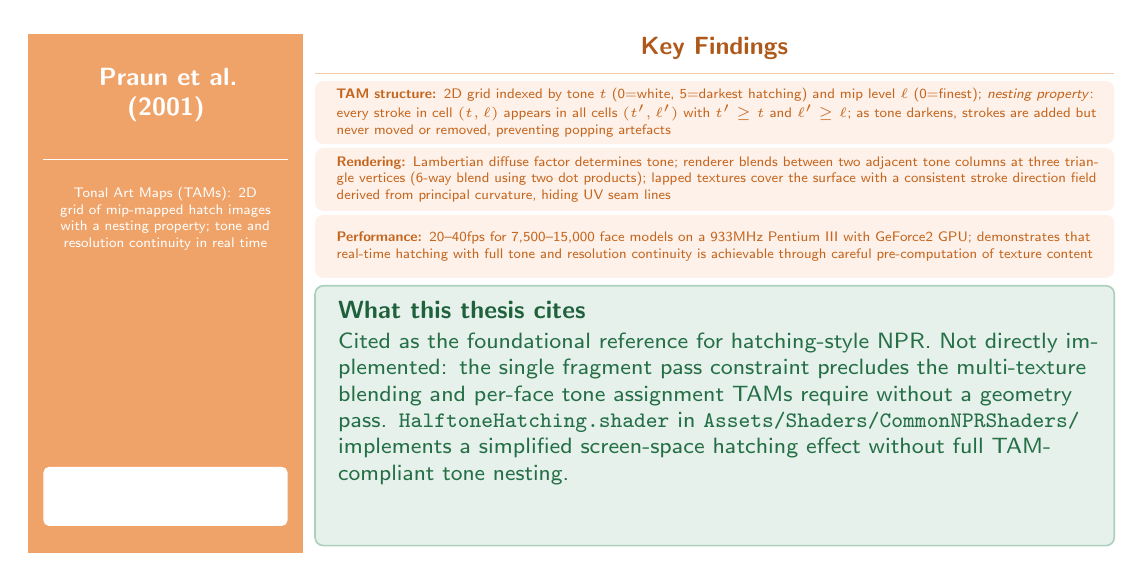
\begin{tikzpicture}[x=1cm, y=1cm]
\fill[korange!68] (0.0,0.0) rectangle (3.5,6.6);
\node[font=\small\sffamily\bfseries, text=white, align=center, text width=3.1cm]
  at (1.75,5.82) {Praun et al.\\(2001)};
\draw[white!30, line width=0.3pt] (0.2,5.00) -- (3.3,5.00);
\node[font=\tiny\sffamily, text=white!85, align=center, text width=3.0cm]
  at (1.75,4.25) {Tonal Art Maps (TAMs): 2D grid of mip-mapped hatch images with a nesting property; tone and resolution continuity in real time};
\fill[white!20, rounded corners=2pt] (0.2,0.35) rectangle (3.3,1.10);
\node[font=\tiny\sffamily\bfseries, text=white, align=center]
  at (1.75,0.72) {SIGGRAPH 2001\\20--40fps on GeForce2};
\node[font=\small\sffamily\bfseries\color{korange!75!black}] at (8.72,6.42) {Key Findings};
\draw[korange!40, line width=0.3pt] (3.65,6.10) -- (13.8,6.10);
\fill[korange!10, rounded corners=3pt] (3.65,5.20) rectangle (13.8,6.00);
\node[font=\tiny\sffamily\color{korange!85!black}, anchor=west, text width=9.65cm]
  at (3.80,5.60) {\textbf{TAM structure:} 2D grid indexed by tone $t$ (0=white, 5=darkest hatching) and mip level $\ell$ (0=finest); \textit{nesting property}: every stroke in cell $(t,\ell)$ appears in all cells $(t',\ell')$ with $t'\geq t$ and $\ell'\geq\ell$; as tone darkens, strokes are added but never moved or removed, preventing popping artefacts};
\fill[korange!10, rounded corners=3pt] (3.65,4.35) rectangle (13.8,5.15);
\node[font=\tiny\sffamily\color{korange!85!black}, anchor=west, text width=9.65cm]
  at (3.80,4.75) {\textbf{Rendering:} Lambertian diffuse factor determines tone; renderer blends between two adjacent tone columns at three triangle vertices (6-way blend using two dot products); lapped textures cover the surface with a consistent stroke direction field derived from principal curvature, hiding UV seam lines};
\fill[korange!10, rounded corners=3pt] (3.65,3.50) rectangle (13.8,4.30);
\node[font=\tiny\sffamily\color{korange!85!black}, anchor=west, text width=9.65cm]
  at (3.80,3.90) {\textbf{Performance:} 20--40fps for 7,500--15,000 face models on a 933MHz Pentium III with GeForce2 GPU; demonstrates that real-time hatching with full tone and resolution continuity is achievable through careful pre-computation of texture content};
\fill[kgreen!12, draw=kgreen!40, rounded corners=3pt, line width=0.6pt]
  (3.65,0.1) rectangle (13.8,3.40);
\node[font=\small\sffamily\bfseries\color{kgreen!70!black}, anchor=west]
  at (3.82,3.1) {What this thesis cites};
\node[font=\footnotesize\sffamily\color{kgreen!80!black}, anchor=north west, text width=9.65cm]
  at (3.82,2.92) {Cited as the foundational reference for hatching-style NPR. Not directly implemented: the single fragment pass constraint precludes the multi-texture blending and per-face tone assignment TAMs require without a geometry pass. \texttt{HalftoneHatching.shader} in \texttt{Assets/Shaders/CommonNPRShaders/} implements a simplified screen-space hatching effect without full TAM-compliant tone nesting.};
\end{tikzpicture}
\end{center}
\end{frame}

%% ═══════════════════════════════════════════════════════════════════════════
%% Roberts 1963
%% ═══════════════════════════════════════════════════════════════════════════
\begin{frame}{Roberts (1963) \textnormal{\normalsize --- Machine Perception of Three-Dimensional Solids}}
\begin{center}
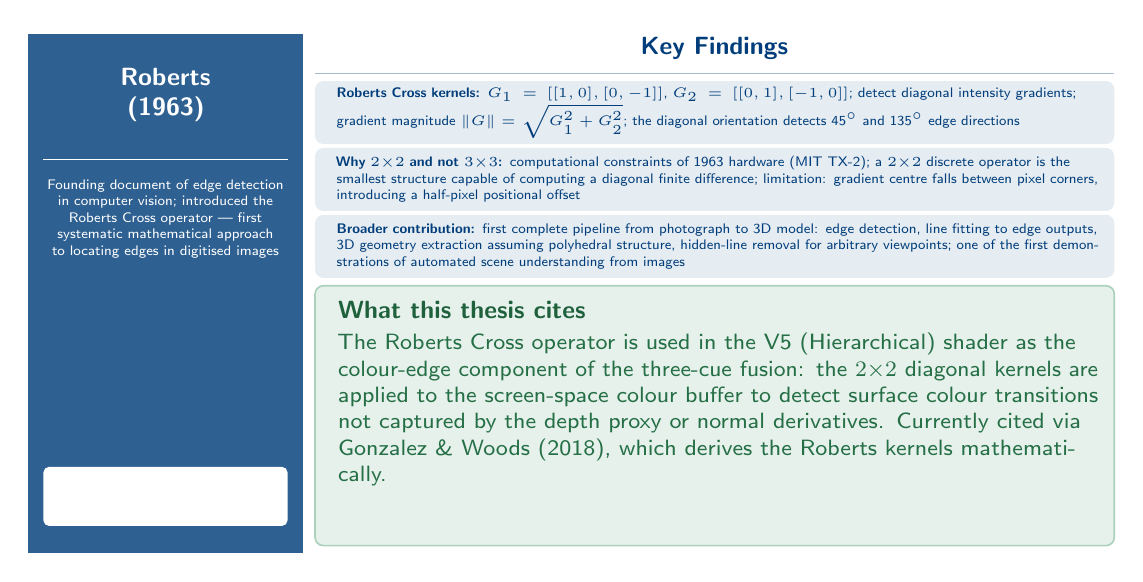
\begin{tikzpicture}[x=1cm, y=1cm]
\fill[kbluedark!82] (0.0,0.0) rectangle (3.5,6.6);
\node[font=\small\sffamily\bfseries, text=white, align=center, text width=3.1cm]
  at (1.75,5.82) {Roberts\\(1963)};
\draw[white!30, line width=0.3pt] (0.2,5.00) -- (3.3,5.00);
\node[font=\tiny\sffamily, text=white!85, align=center, text width=3.0cm]
  at (1.75,4.25) {Founding document of edge detection in computer vision; introduced the Roberts Cross operator --- first systematic mathematical approach to locating edges in digitised images};
\fill[white!20, rounded corners=2pt] (0.2,0.35) rectangle (3.3,1.10);
\node[font=\tiny\sffamily\bfseries, text=white, align=center]
  at (1.75,0.72) {MIT PhD thesis\\Lincoln Lab Report TR-315};
\node[font=\small\sffamily\bfseries\color{kbluedark}] at (8.72,6.42) {Key Findings};
\draw[kbluedark!35, line width=0.3pt] (3.65,6.10) -- (13.8,6.10);
\fill[kbluedark!10, rounded corners=3pt] (3.65,5.20) rectangle (13.8,6.00);
\node[font=\tiny\sffamily\color{kbluedark}, anchor=west, text width=9.65cm]
  at (3.80,5.60) {\textbf{Roberts Cross kernels:} $G_1=[[1,0],[0,-1]]$, $G_2=[[0,1],[-1,0]]$; detect diagonal intensity gradients; gradient magnitude $\|G\| = \sqrt{G_1^2+G_2^2}$; the diagonal orientation detects 45$^\circ$ and 135$^\circ$ edge directions};
\fill[kbluedark!10, rounded corners=3pt] (3.65,4.35) rectangle (13.8,5.15);
\node[font=\tiny\sffamily\color{kbluedark}, anchor=west, text width=9.65cm]
  at (3.80,4.75) {\textbf{Why $2{\times}2$ and not $3{\times}3$:} computational constraints of 1963 hardware (MIT TX-2); a $2{\times}2$ discrete operator is the smallest structure capable of computing a diagonal finite difference; limitation: gradient centre falls between pixel corners, introducing a half-pixel positional offset};
\fill[kbluedark!10, rounded corners=3pt] (3.65,3.50) rectangle (13.8,4.30);
\node[font=\tiny\sffamily\color{kbluedark}, anchor=west, text width=9.65cm]
  at (3.80,3.90) {\textbf{Broader contribution:} first complete pipeline from photograph to 3D model: edge detection, line fitting to edge outputs, 3D geometry extraction assuming polyhedral structure, hidden-line removal for arbitrary viewpoints; one of the first demonstrations of automated scene understanding from images};
\fill[kgreen!12, draw=kgreen!40, rounded corners=3pt, line width=0.6pt]
  (3.65,0.1) rectangle (13.8,3.40);
\node[font=\small\sffamily\bfseries\color{kgreen!70!black}, anchor=west]
  at (3.82,3.1) {What this thesis cites};
\node[font=\footnotesize\sffamily\color{kgreen!80!black}, anchor=north west, text width=9.65cm]
  at (3.82,2.92) {The Roberts Cross operator is used in the V5 (Hierarchical) shader as the colour-edge component of the three-cue fusion: the $2{\times}2$ diagonal kernels are applied to the screen-space colour buffer to detect surface colour transitions not captured by the depth proxy or normal derivatives. Currently cited via Gonzalez \& Woods (2018), which derives the Roberts kernels mathematically.};
\end{tikzpicture}
\end{center}
\end{frame}

%% ═══════════════════════════════════════════════════════════════════════════
%% Kumar & Poornima 2019
%% ═══════════════════════════════════════════════════════════════════════════
\begin{frame}{Kumar \& Poornima (2019) \textnormal{\normalsize --- Comprehensive Survey on Nonphotorealistic Rendering}}
\begin{center}
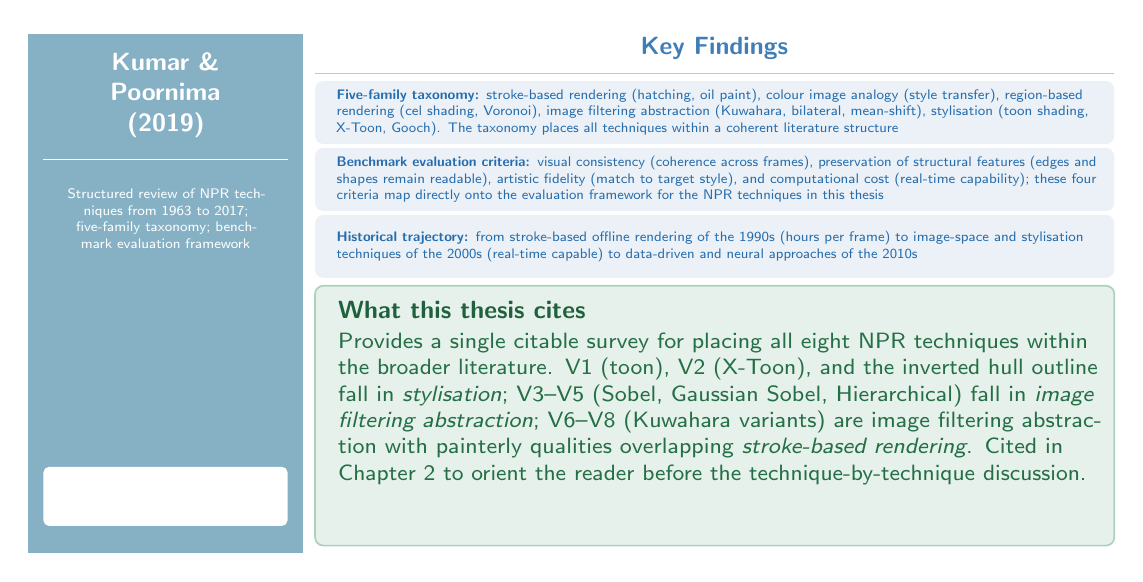
\begin{tikzpicture}[x=1cm, y=1cm]
\fill[kblue!72!kgreen!50] (0.0,0.0) rectangle (3.5,6.6);
\node[font=\small\sffamily\bfseries, text=white, align=center, text width=3.1cm]
  at (1.75,5.82) {Kumar \&\\Poornima\\(2019)};
\draw[white!30, line width=0.3pt] (0.2,5.00) -- (3.3,5.00);
\node[font=\tiny\sffamily, text=white!85, align=center, text width=3.0cm]
  at (1.75,4.25) {Structured review of NPR techniques from 1963 to 2017; five-family taxonomy; benchmark evaluation framework};
\fill[white!20, rounded corners=2pt] (0.2,0.35) rectangle (3.3,1.10);
\node[font=\tiny\sffamily\bfseries, text=white, align=center]
  at (1.75,0.72) {Iran J. Computer Science\\Springer Nature};
\node[font=\small\sffamily\bfseries\color{kblue!75}] at (8.72,6.42) {Key Findings};
\draw[kblue!30, line width=0.3pt] (3.65,6.10) -- (13.8,6.10);
\fill[kblue!8, rounded corners=3pt] (3.65,5.20) rectangle (13.8,6.00);
\node[font=\tiny\sffamily\color{kblue!85}, anchor=west, text width=9.65cm]
  at (3.80,5.60) {\textbf{Five-family taxonomy:} stroke-based rendering (hatching, oil paint), colour image analogy (style transfer), region-based rendering (cel shading, Voronoi), image filtering abstraction (Kuwahara, bilateral, mean-shift), stylisation (toon shading, X-Toon, Gooch). The taxonomy places all techniques within a coherent literature structure};
\fill[kblue!8, rounded corners=3pt] (3.65,4.35) rectangle (13.8,5.15);
\node[font=\tiny\sffamily\color{kblue!85}, anchor=west, text width=9.65cm]
  at (3.80,4.75) {\textbf{Benchmark evaluation criteria:} visual consistency (coherence across frames), preservation of structural features (edges and shapes remain readable), artistic fidelity (match to target style), and computational cost (real-time capability); these four criteria map directly onto the evaluation framework for the NPR techniques in this thesis};
\fill[kblue!8, rounded corners=3pt] (3.65,3.50) rectangle (13.8,4.30);
\node[font=\tiny\sffamily\color{kblue!85}, anchor=west, text width=9.65cm]
  at (3.80,3.90) {\textbf{Historical trajectory:} from stroke-based offline rendering of the 1990s (hours per frame) to image-space and stylisation techniques of the 2000s (real-time capable) to data-driven and neural approaches of the 2010s};
\fill[kgreen!12, draw=kgreen!40, rounded corners=3pt, line width=0.6pt]
  (3.65,0.1) rectangle (13.8,3.40);
\node[font=\small\sffamily\bfseries\color{kgreen!70!black}, anchor=west]
  at (3.82,3.1) {What this thesis cites};
\node[font=\footnotesize\sffamily\color{kgreen!80!black}, anchor=north west, text width=9.65cm]
  at (3.82,2.92) {Provides a single citable survey for placing all eight NPR techniques within the broader literature. V1 (toon), V2 (X-Toon), and the inverted hull outline fall in \textit{stylisation}; V3--V5 (Sobel, Gaussian Sobel, Hierarchical) fall in \textit{image filtering abstraction}; V6--V8 (Kuwahara variants) are image filtering abstraction with painterly qualities overlapping \textit{stroke-based rendering}. Cited in Chapter 2 to orient the reader before the technique-by-technique discussion.};
\end{tikzpicture}
\end{center}
\end{frame}

%% ═══════════════════════════════════════════════════════════════════════════
%% Wisessing, Dingliana & McDonnell 2016
%% ═══════════════════════════════════════════════════════════════════════════
\begin{frame}{Wisessing, Dingliana \& McDonnell (2016) \textnormal{\normalsize --- Perception of Lighting and Shading for Animated Characters}}
\begin{center}
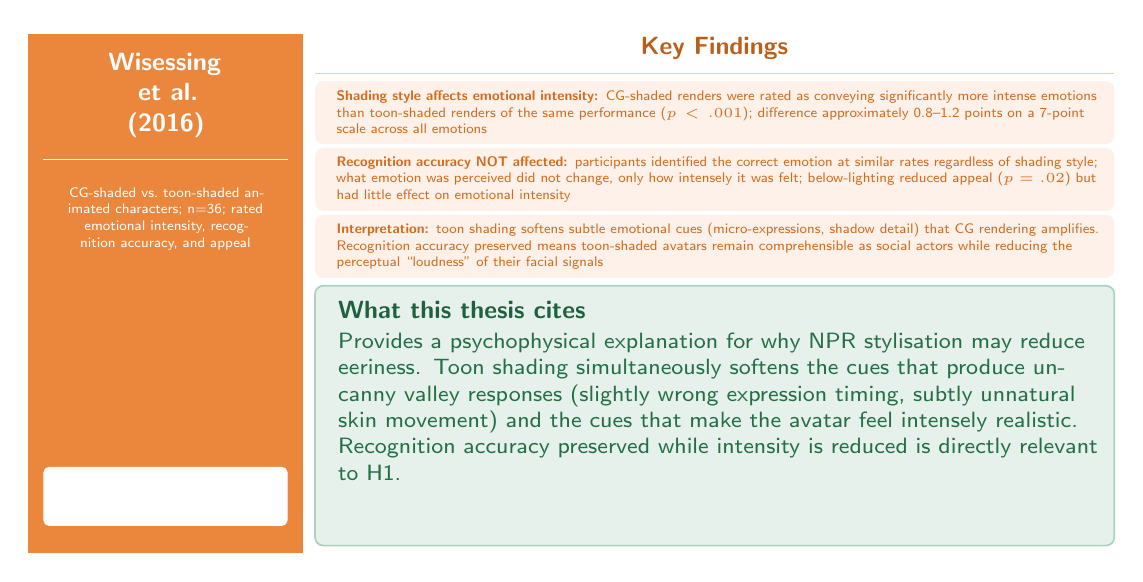
\begin{tikzpicture}[x=1cm, y=1cm]
\fill[korange!88] (0.0,0.0) rectangle (3.5,6.6);
\node[font=\small\sffamily\bfseries, text=white, align=center, text width=3.1cm]
  at (1.75,5.82) {Wisessing\\et al.\\(2016)};
\draw[white!30, line width=0.3pt] (0.2,5.00) -- (3.3,5.00);
\node[font=\tiny\sffamily, text=white!85, align=center, text width=3.0cm]
  at (1.75,4.25) {CG-shaded vs.\ toon-shaded animated characters; n=36; rated emotional intensity, recognition accuracy, and appeal};
\fill[white!20, rounded corners=2pt] (0.2,0.35) rectangle (3.3,1.10);
\node[font=\tiny\sffamily\bfseries, text=white, align=center]
  at (1.75,0.72) {ACM SAP 2016\\empirical, n = 36};
\node[font=\small\sffamily\bfseries\color{korange!80!black}] at (8.72,6.42) {Key Findings};
\draw[korange!40, line width=0.3pt] (3.65,6.10) -- (13.8,6.10);
\fill[korange!10, rounded corners=3pt] (3.65,5.20) rectangle (13.8,6.00);
\node[font=\tiny\sffamily\color{korange!90!black}, anchor=west, text width=9.65cm]
  at (3.80,5.60) {\textbf{Shading style affects emotional intensity:} CG-shaded renders were rated as conveying significantly more intense emotions than toon-shaded renders of the same performance ($p < .001$); difference approximately 0.8--1.2 points on a 7-point scale across all emotions};
\fill[korange!10, rounded corners=3pt] (3.65,4.35) rectangle (13.8,5.15);
\node[font=\tiny\sffamily\color{korange!90!black}, anchor=west, text width=9.65cm]
  at (3.80,4.75) {\textbf{Recognition accuracy NOT affected:} participants identified the correct emotion at similar rates regardless of shading style; what emotion was perceived did not change, only how intensely it was felt; below-lighting reduced appeal ($p = .02$) but had little effect on emotional intensity};
\fill[korange!10, rounded corners=3pt] (3.65,3.50) rectangle (13.8,4.30);
\node[font=\tiny\sffamily\color{korange!90!black}, anchor=west, text width=9.65cm]
  at (3.80,3.90) {\textbf{Interpretation:} toon shading softens subtle emotional cues (micro-expressions, shadow detail) that CG rendering amplifies. Recognition accuracy preserved means toon-shaded avatars remain comprehensible as social actors while reducing the perceptual ``loudness'' of their facial signals};
\fill[kgreen!12, draw=kgreen!40, rounded corners=3pt, line width=0.6pt]
  (3.65,0.1) rectangle (13.8,3.40);
\node[font=\small\sffamily\bfseries\color{kgreen!70!black}, anchor=west]
  at (3.82,3.1) {What this thesis cites};
\node[font=\footnotesize\sffamily\color{kgreen!80!black}, anchor=north west, text width=9.65cm]
  at (3.82,2.92) {Provides a psychophysical explanation for why NPR stylisation may reduce eeriness. Toon shading simultaneously softens the cues that produce uncanny valley responses (slightly wrong expression timing, subtly unnatural skin movement) and the cues that make the avatar feel intensely realistic. Recognition accuracy preserved while intensity is reduced is directly relevant to H1.};
\end{tikzpicture}
\end{center}
\end{frame}

%% ═══════════════════════════════════════════════════════════════════════════
%% Wisessing et al. 2020
%% ═══════════════════════════════════════════════════════════════════════════
\begin{frame}{Wisessing et al. (2020) \textnormal{\normalsize --- Enlighten Me: Brightness and Shadow for Character Emotion and Appeal}}
\begin{center}
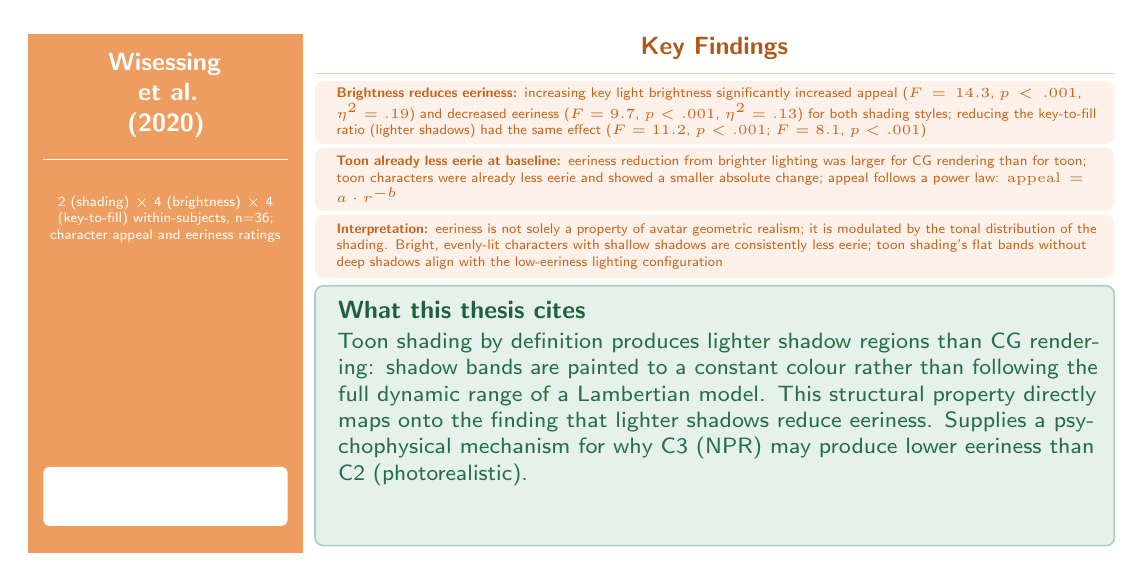
\begin{tikzpicture}[x=1cm, y=1cm]
\fill[korange!72] (0.0,0.0) rectangle (3.5,6.6);
\node[font=\small\sffamily\bfseries, text=white, align=center, text width=3.1cm]
  at (1.75,5.82) {Wisessing\\et al.\\(2020)};
\draw[white!30, line width=0.3pt] (0.2,5.00) -- (3.3,5.00);
\node[font=\tiny\sffamily, text=white!85, align=center, text width=3.0cm]
  at (1.75,4.25) {2 (shading) $\times$ 4 (brightness) $\times$ 4 (key-to-fill) within-subjects, n=36; character appeal and eeriness ratings};
\fill[white!20, rounded corners=2pt] (0.2,0.35) rectangle (3.3,1.10);
\node[font=\tiny\sffamily\bfseries, text=white, align=center]
  at (1.75,0.72) {ACM Trans.\ Graphics\\follow-up to SAP 2016};
\node[font=\small\sffamily\bfseries\color{korange!75!black}] at (8.72,6.42) {Key Findings};
\draw[korange!40, line width=0.3pt] (3.65,6.10) -- (13.8,6.10);
\fill[korange!10, rounded corners=3pt] (3.65,5.20) rectangle (13.8,6.00);
\node[font=\tiny\sffamily\color{korange!85!black}, anchor=west, text width=9.65cm]
  at (3.80,5.60) {\textbf{Brightness reduces eeriness:} increasing key light brightness significantly increased appeal ($F=14.3$, $p<.001$, $\eta^2=.19$) and decreased eeriness ($F=9.7$, $p<.001$, $\eta^2=.13$) for both shading styles; reducing the key-to-fill ratio (lighter shadows) had the same effect ($F=11.2$, $p<.001$; $F=8.1$, $p<.001$)};
\fill[korange!10, rounded corners=3pt] (3.65,4.35) rectangle (13.8,5.15);
\node[font=\tiny\sffamily\color{korange!85!black}, anchor=west, text width=9.65cm]
  at (3.80,4.75) {\textbf{Toon already less eerie at baseline:} eeriness reduction from brighter lighting was larger for CG rendering than for toon; toon characters were already less eerie and showed a smaller absolute change; appeal follows a power law: $\mathrm{appeal} = a \cdot r^{-b}$};
\fill[korange!10, rounded corners=3pt] (3.65,3.50) rectangle (13.8,4.30);
\node[font=\tiny\sffamily\color{korange!85!black}, anchor=west, text width=9.65cm]
  at (3.80,3.90) {\textbf{Interpretation:} eeriness is not solely a property of avatar geometric realism; it is modulated by the tonal distribution of the shading. Bright, evenly-lit characters with shallow shadows are consistently less eerie; toon shading's flat bands without deep shadows align with the low-eeriness lighting configuration};
\fill[kgreen!12, draw=kgreen!40, rounded corners=3pt, line width=0.6pt]
  (3.65,0.1) rectangle (13.8,3.40);
\node[font=\small\sffamily\bfseries\color{kgreen!70!black}, anchor=west]
  at (3.82,3.1) {What this thesis cites};
\node[font=\footnotesize\sffamily\color{kgreen!80!black}, anchor=north west, text width=9.65cm]
  at (3.82,2.92) {Toon shading by definition produces lighter shadow regions than CG rendering: shadow bands are painted to a constant colour rather than following the full dynamic range of a Lambertian model. This structural property directly maps onto the finding that lighter shadows reduce eeriness. Supplies a psychophysical mechanism for why C3 (NPR) may produce lower eeriness than C2 (photorealistic).};
\end{tikzpicture}
\end{center}
\end{frame}

%% ═══════════════════════════════════════════════════════════════════════════
%% Petikam, Anjyo & Rhee 2021
%% ═══════════════════════════════════════════════════════════════════════════
\begin{frame}{Petikam, Anjyo \& Rhee (2021) \textnormal{\normalsize --- Shading Rig: Art-Directable Stylised Shading for 3D Characters}}
\begin{center}
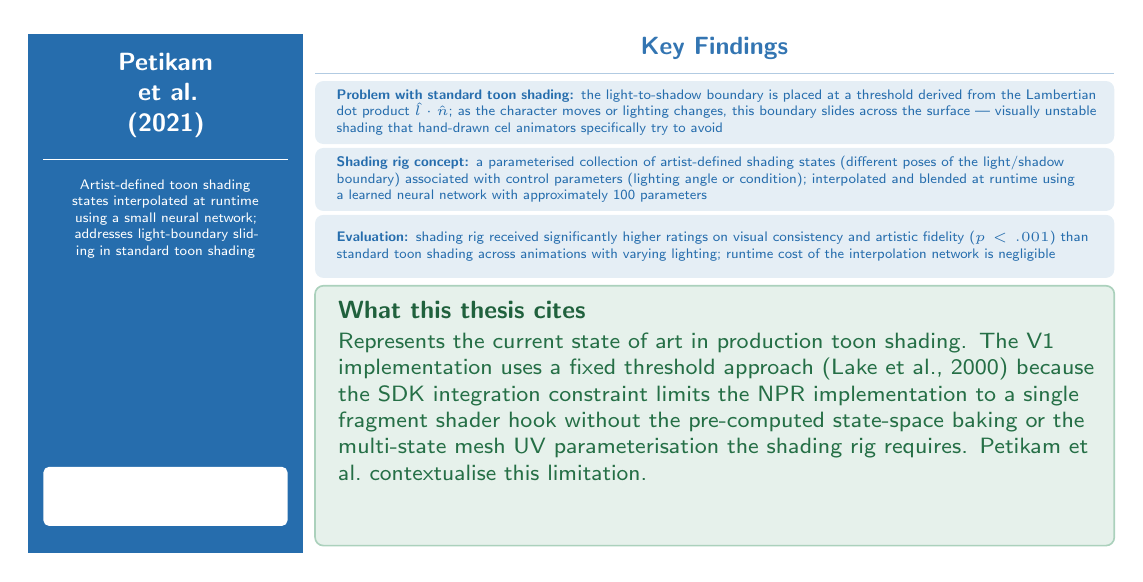
\begin{tikzpicture}[x=1cm, y=1cm]
\fill[kblue!85] (0.0,0.0) rectangle (3.5,6.6);
\node[font=\small\sffamily\bfseries, text=white, align=center, text width=3.1cm]
  at (1.75,5.82) {Petikam\\et al.\\(2021)};
\draw[white!30, line width=0.3pt] (0.2,5.00) -- (3.3,5.00);
\node[font=\tiny\sffamily, text=white!85, align=center, text width=3.0cm]
  at (1.75,4.25) {Artist-defined toon shading states interpolated at runtime using a small neural network; addresses light-boundary sliding in standard toon shading};
\fill[white!20, rounded corners=2pt] (0.2,0.35) rectangle (3.3,1.10);
\node[font=\tiny\sffamily\bfseries, text=white, align=center]
  at (1.75,0.72) {ACM Trans.\ Graphics\\user study n = 26};
\node[font=\small\sffamily\bfseries\color{kblue!80}] at (8.72,6.42) {Key Findings};
\draw[kblue!30, line width=0.3pt] (3.65,6.10) -- (13.8,6.10);
\fill[kblue!10, rounded corners=3pt] (3.65,5.20) rectangle (13.8,6.00);
\node[font=\tiny\sffamily\color{kblue!85}, anchor=west, text width=9.65cm]
  at (3.80,5.60) {\textbf{Problem with standard toon shading:} the light-to-shadow boundary is placed at a threshold derived from the Lambertian dot product $\hat{l}\cdot\hat{n}$; as the character moves or lighting changes, this boundary slides across the surface --- visually unstable shading that hand-drawn cel animators specifically try to avoid};
\fill[kblue!10, rounded corners=3pt] (3.65,4.35) rectangle (13.8,5.15);
\node[font=\tiny\sffamily\color{kblue!85}, anchor=west, text width=9.65cm]
  at (3.80,4.75) {\textbf{Shading rig concept:} a parameterised collection of artist-defined shading states (different poses of the light/shadow boundary) associated with control parameters (lighting angle or condition); interpolated and blended at runtime using a learned neural network with approximately 100 parameters};
\fill[kblue!10, rounded corners=3pt] (3.65,3.50) rectangle (13.8,4.30);
\node[font=\tiny\sffamily\color{kblue!85}, anchor=west, text width=9.65cm]
  at (3.80,3.90) {\textbf{Evaluation:} shading rig received significantly higher ratings on visual consistency and artistic fidelity ($p<.001$) than standard toon shading across animations with varying lighting; runtime cost of the interpolation network is negligible};
\fill[kgreen!12, draw=kgreen!40, rounded corners=3pt, line width=0.6pt]
  (3.65,0.1) rectangle (13.8,3.40);
\node[font=\small\sffamily\bfseries\color{kgreen!70!black}, anchor=west]
  at (3.82,3.1) {What this thesis cites};
\node[font=\footnotesize\sffamily\color{kgreen!80!black}, anchor=north west, text width=9.65cm]
  at (3.82,2.92) {Represents the current state of art in production toon shading. The V1 implementation uses a fixed threshold approach (Lake et al., 2000) because the SDK integration constraint limits the NPR implementation to a single fragment shader hook without the pre-computed state-space baking or the multi-state mesh UV parameterisation the shading rig requires. Petikam et al.\ contextualise this limitation.};
\end{tikzpicture}
\end{center}
\end{frame}

%% ═══════════════════════════════════════════════════════════════════════════
%% Riefard et al. 2024
%% ═══════════════════════════════════════════════════════════════════════════
\begin{frame}{Riefard et al. (2024) \textnormal{\normalsize --- Player Preferences for NPR Artistic Styles in 3D Game Characters}}
\begin{center}
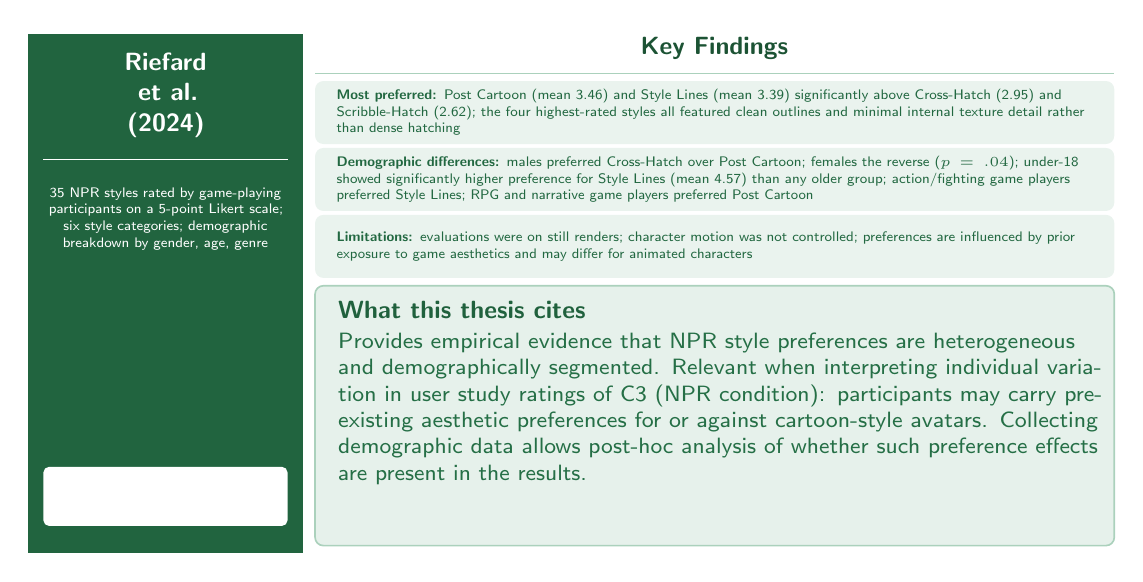
\begin{tikzpicture}[x=1cm, y=1cm]
\fill[kgreen!72!black] (0.0,0.0) rectangle (3.5,6.6);
\node[font=\small\sffamily\bfseries, text=white, align=center, text width=3.1cm]
  at (1.75,5.82) {Riefard\\et al.\\(2024)};
\draw[white!30, line width=0.3pt] (0.2,5.00) -- (3.3,5.00);
\node[font=\tiny\sffamily, text=white!85, align=center, text width=3.0cm]
  at (1.75,4.25) {35 NPR styles rated by game-playing participants on a 5-point Likert scale; six style categories; demographic breakdown by gender, age, genre};
\fill[white!20, rounded corners=2pt] (0.2,0.35) rectangle (3.3,1.10);
\node[font=\tiny\sffamily\bfseries, text=white, align=center]
  at (1.75,0.72) {ICECOS 2024\\IEEE survey study};
\node[font=\small\sffamily\bfseries\color{kgreen!60!black}] at (8.72,6.42) {Key Findings};
\draw[kgreen!40, line width=0.3pt] (3.65,6.10) -- (13.8,6.10);
\fill[kgreen!10, rounded corners=3pt] (3.65,5.20) rectangle (13.8,6.00);
\node[font=\tiny\sffamily\color{kgreen!75!black}, anchor=west, text width=9.65cm]
  at (3.80,5.60) {\textbf{Most preferred:} Post Cartoon (mean 3.46) and Style Lines (mean 3.39) significantly above Cross-Hatch (2.95) and Scribble-Hatch (2.62); the four highest-rated styles all featured clean outlines and minimal internal texture detail rather than dense hatching};
\fill[kgreen!10, rounded corners=3pt] (3.65,4.35) rectangle (13.8,5.15);
\node[font=\tiny\sffamily\color{kgreen!75!black}, anchor=west, text width=9.65cm]
  at (3.80,4.75) {\textbf{Demographic differences:} males preferred Cross-Hatch over Post Cartoon; females the reverse ($p=.04$); under-18 showed significantly higher preference for Style Lines (mean 4.57) than any older group; action/fighting game players preferred Style Lines; RPG and narrative game players preferred Post Cartoon};
\fill[kgreen!10, rounded corners=3pt] (3.65,3.50) rectangle (13.8,4.30);
\node[font=\tiny\sffamily\color{kgreen!75!black}, anchor=west, text width=9.65cm]
  at (3.80,3.90) {\textbf{Limitations:} evaluations were on still renders; character motion was not controlled; preferences are influenced by prior exposure to game aesthetics and may differ for animated characters};
\fill[kgreen!12, draw=kgreen!40, rounded corners=3pt, line width=0.6pt]
  (3.65,0.1) rectangle (13.8,3.40);
\node[font=\small\sffamily\bfseries\color{kgreen!70!black}, anchor=west]
  at (3.82,3.1) {What this thesis cites};
\node[font=\footnotesize\sffamily\color{kgreen!80!black}, anchor=north west, text width=9.65cm]
  at (3.82,2.92) {Provides empirical evidence that NPR style preferences are heterogeneous and demographically segmented. Relevant when interpreting individual variation in user study ratings of C3 (NPR condition): participants may carry pre-existing aesthetic preferences for or against cartoon-style avatars. Collecting demographic data allows post-hoc analysis of whether such preference effects are present in the results.};
\end{tikzpicture}
\end{center}
\end{frame}

%% ═══════════════════════════════════════════════════════════════════════════
%% Roshaan 2026 — AHEAD
%% ═══════════════════════════════════════════════════════════════════════════
\begin{frame}{Roshaan (2026, preprint) \textnormal{\normalsize --- AHEAD: Adaptive Hierarchical Edge Detection}}
\begin{center}
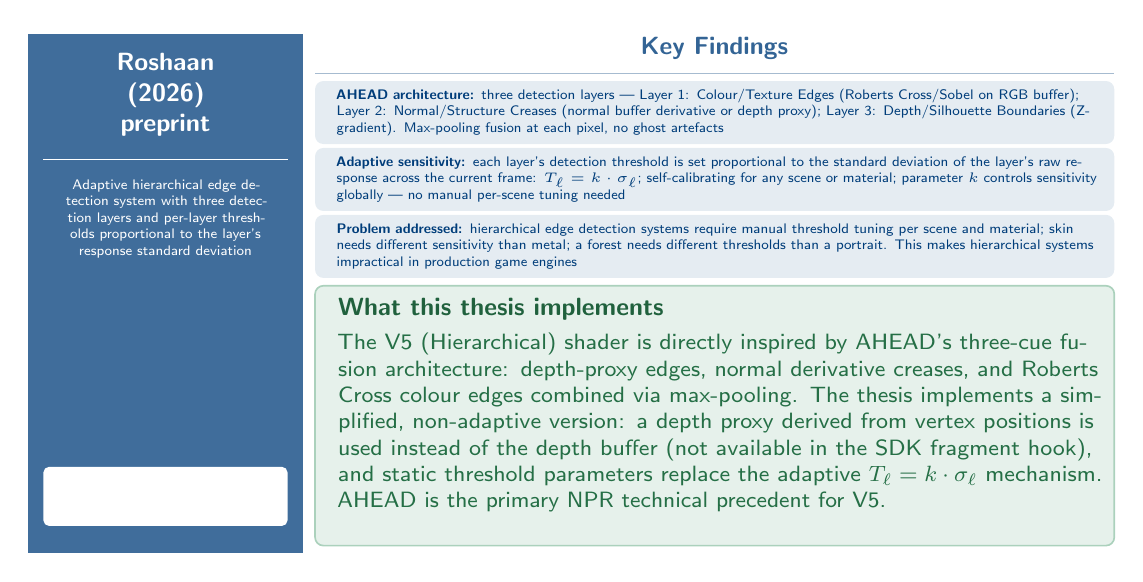
\begin{tikzpicture}[x=1cm, y=1cm]
\fill[kbluedark!75] (0.0,0.0) rectangle (3.5,6.6);
\node[font=\small\sffamily\bfseries, text=white, align=center, text width=3.1cm]
  at (1.75,5.82) {Roshaan\\(2026)\\preprint};
\draw[white!30, line width=0.3pt] (0.2,5.00) -- (3.3,5.00);
\node[font=\tiny\sffamily, text=white!85, align=center, text width=3.0cm]
  at (1.75,4.25) {Adaptive hierarchical edge detection system with three detection layers and per-layer thresholds proportional to the layer's response standard deviation};
\fill[white!20, rounded corners=2pt] (0.2,0.35) rectangle (3.3,1.10);
\node[font=\tiny\sffamily\bfseries, text=white, align=center]
  at (1.75,0.72) {Research Square preprint\\real-time shader};
\node[font=\small\sffamily\bfseries\color{kbluedark!80}] at (8.72,6.42) {Key Findings};
\draw[kbluedark!35, line width=0.3pt] (3.65,6.10) -- (13.8,6.10);
\fill[kbluedark!10, rounded corners=3pt] (3.65,5.20) rectangle (13.8,6.00);
\node[font=\tiny\sffamily\color{kbluedark}, anchor=west, text width=9.65cm]
  at (3.80,5.60) {\textbf{AHEAD architecture:} three detection layers --- Layer 1: Colour/Texture Edges (Roberts Cross/Sobel on RGB buffer); Layer 2: Normal/Structure Creases (normal buffer derivative or depth proxy); Layer 3: Depth/Silhouette Boundaries (Z-gradient). Max-pooling fusion at each pixel, no ghost artefacts};
\fill[kbluedark!10, rounded corners=3pt] (3.65,4.35) rectangle (13.8,5.15);
\node[font=\tiny\sffamily\color{kbluedark}, anchor=west, text width=9.65cm]
  at (3.80,4.75) {\textbf{Adaptive sensitivity:} each layer's detection threshold is set proportional to the standard deviation of the layer's raw response across the current frame: $T_\ell = k \cdot \sigma_\ell$; self-calibrating for any scene or material; parameter $k$ controls sensitivity globally --- no manual per-scene tuning needed};
\fill[kbluedark!10, rounded corners=3pt] (3.65,3.50) rectangle (13.8,4.30);
\node[font=\tiny\sffamily\color{kbluedark}, anchor=west, text width=9.65cm]
  at (3.80,3.90) {\textbf{Problem addressed:} hierarchical edge detection systems require manual threshold tuning per scene and material; skin needs different sensitivity than metal; a forest needs different thresholds than a portrait. This makes hierarchical systems impractical in production game engines};
\fill[kgreen!12, draw=kgreen!40, rounded corners=3pt, line width=0.6pt]
  (3.65,0.1) rectangle (13.8,3.40);
\node[font=\small\sffamily\bfseries\color{kgreen!70!black}, anchor=west]
  at (3.82,3.1) {What this thesis implements};
\node[font=\footnotesize\sffamily\color{kgreen!80!black}, anchor=north west, text width=9.65cm]
  at (3.82,2.92) {The V5 (Hierarchical) shader is directly inspired by AHEAD's three-cue fusion architecture: depth-proxy edges, normal derivative creases, and Roberts Cross colour edges combined via max-pooling. The thesis implements a simplified, non-adaptive version: a depth proxy derived from vertex positions is used instead of the depth buffer (not available in the SDK fragment hook), and static threshold parameters replace the adaptive $T_\ell = k\cdot\sigma_\ell$ mechanism. AHEAD is the primary NPR technical precedent for V5.};
\end{tikzpicture}
\end{center}
\end{frame}

\end{document}
